\section{CPV in D-meson system}

The quark constituents of the $D^{0}(1865)$ and $\bar{D}^{0}(1865)$ mesons are $(c \bar{u})$ and $(u \bar{c})$, respectively. This system is unique as it is the only system which undergoes mixing and contains an up-type quark. As opposed to the $K^{0}$,$B^{0}$ and $B_{S}$, which contain down quarks. This results in different quarks in the mixing box diagrams of these processes, which are illustrated in Fig.(\ref{KevFeyn1.png}) and (\ref{Deon_Mixing_Feyn}). The rates for $D^0$ mixing are expected to be very small as the mixing process shown is suppressed in two ways. If the intermediate quark is a b, then the decay is doubly Cabbibo suppressed[explain? or has it been explained already?], while if the quark is a d or an s then the process is GIM suppressed[Reference John]. Other processes which may not have the same degree of suppression have been proposed, but there are large incertainties in the theoretical calculations of their decay rates \cite{Babar_D0_Review}.    

\begin{figure}[h!]
\begin{center}
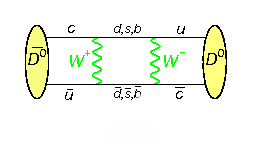
\includegraphics[scale=0.8]{figs/Deon_mixing_feyn.png}
\end{center}
\caption{\textit{Feynmann diagram showing the process by which the two $D^{0}$ states mix. This process is the only known mixing process which contain the d,s,b quarks in this position \cite{Deon_Mixing_Feyn}}}
\label{Deon_Mixing_Feyn}
\end{figure}

The first stage in detecting CPV in any system is to find mixing between a particle and its anti-particle. Clear evidence for mixing between these states was announced in 2007 and published in 2008 by the BaBar collaboration, followed shortly by the Belle collaboration \cite{BabarD0mixing}\cite{BelleD0mixing}. Results from both experiments show a small amount of $D^{0}$ mixing with 3.9 $\sigma$ certainty, at a level which is consistent with SM predictions in the order of $|x|,|y| \leq \e{-2}$, see Eqn.(\ref{xyDeonMixing}) \cite{Babar_D0_Review}. However, measured CP violating parameters were consistent with zero, and thus with no CPV. We now discuss the Babar experiment.

Two decays and their corresponding anti-particle decays were important for the BaBar measurment of mixing in the D-meson system. The doubly Cabbibo suppressed (DCS) $D^{0} \rightarrow K^{+} \pi^{-}$ known as the wrong sign (WS) decay and $D^{0} \rightarrow K^{-} \pi^{+}$ Cabbibo favoured (CF) decay called the right sign (RS), were used. Two parameters which determine the amount of mixing in a system are defined as:

\begin{align}\label{xyDeonMixing}
x = \frac{\Delta M}{\Gamma} & & y = \frac{\Delta \Gamma}{2 \Gamma}
\end{align}

\noindent where $M= (M_{1}+M_{2})/2$ is average mass,$\Gamma = (\Gamma_{1}+\Gamma_{2})/2$ is average lifetime and $\Delta A \vcentcolon A_{2} - A_{1}$. An approximation to the time dependence of the WS decay in the absence of CPV is given by \cite{BabarD0mixing}:

\begin{equation*}
\frac{T_{WS}(t)}{e^{-\Gamma t}} \propto R_{D} + \sqrt{R_{D}} y \Gamma t + \frac{x^2 + y^2}{4} (\Gamma t)^{2}
\end{equation*}

\noindent Where $R_{D}$ is the ratio of the amplitudes of the DCS decay to to CF deacy. By measuring this time dependence and fitting the results to this formula, we can compare predicted values of x and y from various theoretical models and see which best fits the data. Fig.(\ref{BaBar_D0_Mixing_Results.png}) shows the results of the BaBar experiment. Flavour tagging of the $D^{0}$ is used in this experiment. The sign of a pion known as the ``slow pion'' from the decay $D^{0*} \rightarrow D^{0} \pi^{+}_{s}$ is compared to the sign of the final product Kaon. Where $D^{0*}$ is a heavier, and thus more energetic version of the $D^{0}$ meson. If the signs are the same, the decay is WS, if they are opposite then the decay is RS. Misidentifying a random pion - not from the $D^{0*}$ decay - as the slow pion causes events which do not contain $D^{0}$ decays to be included in analysis. This creates a background which obstructs the signal data. Other sources of background are misreconstructed $D^{0}$ and combinatorial sources. Misreconstruction is due in part to semi-leptonics decays of the $D^{0}$ or $\bar{D}^{0}$ in which the detector has misidentified a lepton as a pion. Combinartorial background is caused by D-mesons being produced not from $D^{0*}$, but from various possible decays of a B-meson. All of these backgrounds are reduced and excluded from the signal decays by making offline cuts to various parameters. These parameters include the the $\chi^{2}$ of the track, vertex and impact parameters of the partilces, the momentum and the mass as well as many others. Mass is plotted in two ways, the reconstructed $D^{0}$ mass distribution $(m_{K \pi})$ and the mass difference between the reconstructed $D^{0*}$ and the $D^{0}$ mass $(\Delta m)$ \cite{Kevin}. We identify signal as events which have a mass peak in the correct place in both $m_{K \pi}$ and $(\Delta m)$, random pion background has a peak in $m_{K \pi}$ but no peak in $(\Delta m)$, and vise versa for misreconstracted particles. Combinatorial background has no peak in either mass distribution. These techniques are of course universal to most particle physics experiemnts. 

\begin{figure}[h!]
\begin{center}
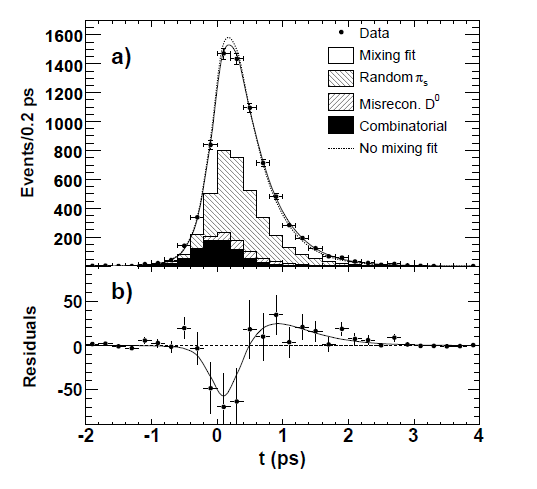
\includegraphics[scale=0.4]{figs/BaBar_D0_Mixing_Results.png}
\end{center}
\caption{\textit{Results from the first $D^{0}$ mixing experiments at BaBar, which plots the time distribution of WS decays. It is clear that the data best fits the mixing hypothesis. Backround contributions from wrongly identified $\pi^{+}_{s}$, misconstructed $D^{0}$ decays and combinatorial contributions from $D^{0}$ production from $B^{0}$ decays are removed}}
\label{BaBar_D0_Mixing_Results.png}
\end{figure}

We discuss here the more recent methods and measurements for mixing parameters. As in the case of Kaon and B-meson mixing we define the CP eigenstates of the D-meson to be linear combinations of flavour eigenstates.

\begin{equation*}
\ket{D^{0}_{1,2}} = p \ket{D^{0}} \pm q \ket{\bar{D}^{0}}
\end{equation*}

\noindent Where for normailzation $|p|^{2}+|q|^{2} = 1$. In the absence of CPV the $\ket{D_{1}}$ state is a CP even state while the $\ket{D_{2}}$ state is a CP odd state. As expected, we will see CPV in mixing if $|p| \neq |q|$. More recent experiments alos use the DCS and CF decays mentioned above. 






These parameters can be measured by considering the decays $D^{0} \rightarrow K^{0}_{s} h^{+} h^{-}$, where $h$ represents either a Kaon or a pion. An intermediate particle $K^{*}$, is constructed from the Kaon and one of the $h$ partilces. In this way, the decay of $K^{*}$ is a two body decay. A Dalitz plot of the mass distributions of the decay products can then be made. This plot has $m^{2}_{K^{*}h^{-}}$ on one axis and $m^{2}_{K^{*}h+}$ on the other axis. These plots are a useful tool for finding resonances in experimental data. For this experiment the total amplitude for the decays mentioned can be written in terms of a superposition of these resonances \cite{Babar_D0_Review}.

\begin{equation*}
A(m^{2}_{K^{*}h^{-}},m^{2}_{K^{*}h^{-}}) = \sum_{r} |A_{R} (m^{2}_{K^{*}h^{-}},m^{2}_{K^{*}h^{-}})| e^{i \phi_{r}} A_{R} (m^{2}_{K^{*}h^{-}},m^{2}_{K^{*}h^{-}}) + a_{NR} r^{i \phi_{NR}}
\end{equation*}

\noindent Where NR represents parameters in a non-resonant term and $\phi$ is a phase. 


The use of ths plot to determine x and y is discussed in \cite{Deon_CopOut}.   
